
Next, we analyze the relative overrepresentation of bidirectional
connections in a network with continuously distributed connection
probabilities. The gamma distribution $\Gamma(\alpha, \beta)$ with
probability density function
\begin{align}
    f_{\alpha,\beta}(x) = \begin{cases} 
\frac{1}{\beta^{\alpha}\Gamma(\alpha)}\, x^{\alpha-1}\,e^{-x/\beta} & x \geq 0 \\
0 & \text{otherwise},
\end{cases}
\end{align}
allows the variation of the variance $\Var(X)= \alpha \beta^2 $ of a
gamma distributed random variable $X \sim \Gamma(\alpha, \beta)$ while
keeping its mean $\E(X) = \alpha \beta $ constant \cite{Hogg1978}.
%\cc{pages 103-105}
The exponential distribution emerges as a special case of the gamma
distribution ($\alpha =1$).

Here we consider a slight modification to the traditional gamma
distribution in the form of a truncated version. Let $\alpha, \beta >
0$. A random variable $X$ follows the truncated gamma distribution
$\Gamma^T(\alpha, \beta)$ if it has the probability density function
%
\begin{align}
  f_{\alpha,\beta}^T(x) = \begin{cases} K_{\alpha, \beta}\,
\frac{1}{\beta^{\alpha}\Gamma(\alpha)}\, x^{\alpha-1}\,e^{-x/\beta} & 0 \leq x \leq 1 \\
0 & \text{otherwise}.
\end{cases}
\end{align}
%
The factor $K_{\alpha,\beta}$ is the inverse of the cumulative
probability $x \leq 1$ of the untruncated gamma distribution,
\begin{align}
  K_{\alpha,\beta} = \left(\int_0^{1} f_{\alpha,\beta}(x) \, dx \right)^{-1},
\end{align}
and is needed to ensure that
\begin{align}
  \int f_{\alpha,\beta}^T(x) \,dx = 1 \label{eq:gd1}.
\end{align}
Consider then the above network model in which the connection
probabilities $P_{ij}$ are $\Gamma^T(\alpha, \beta)$ distributed. We
computed the relative overrepresentation $\varrho$ numerically from
\begin{align}
  \mu = \E(P_{ij}) &= \int_0^1 x f_{\alpha,\beta}^T(x)\, dx,\\
        \E(P_{ij}^2) &= \int_0^1 x^2 f_{\alpha,\beta}^T(x)\, dx.
\end{align}
%
Pairings of the shape parameter $\alpha$ and the scale parameter
$\beta$ were chosen such that the overall connection probability
reflects connectivity statistics in local cortical networks, $\mu =
0.1$. Probability density functions and resulting relative
overrepresentation of reciprocal connections $\varrho$ for four
representative $\alpha,\beta$ pairs are shown in
Figure~\ref{fig:gd}A. Here, $\beta$ was determined to yield $\mu =
0.1$ for the given $\alpha$, following the relationship shown in
Figure~\ref{fig:gd}B.

In the sparse networks we modeled, the truncated gamma distribution
can be well approximated by the untruncated version, $K_{\alpha,
  \beta} \approx 1$. Assuming connections probabilities to be standard
gamma distributed, $P_{ij} \sim \Gamma(\alpha,\beta)$, we have
\begin{align}
  \E(P_{ij}^2) = \Var(P_{ij}) + \E(P_{ij})^2 =  \alpha \beta^2 + \alpha^2 \beta^2, 
\end{align}
and thus
\begin{align}
  \frac{\E(P_{ij}^2)}{\E(P_{ij})^2} = \frac{\alpha^2 \beta^2}{\alpha^2 \beta^2} + \frac{\alpha \beta^2}{\alpha^2 \beta^2} =
 1 + \frac{1}{\alpha}.
\end{align}
The approximation $\varrho = 1 + \frac{1}{\alpha}$ works well for
$\alpha \geq 1$ as shown in Figure~\ref{fig:gd}C.


\begin{figure}[h!]
\centering
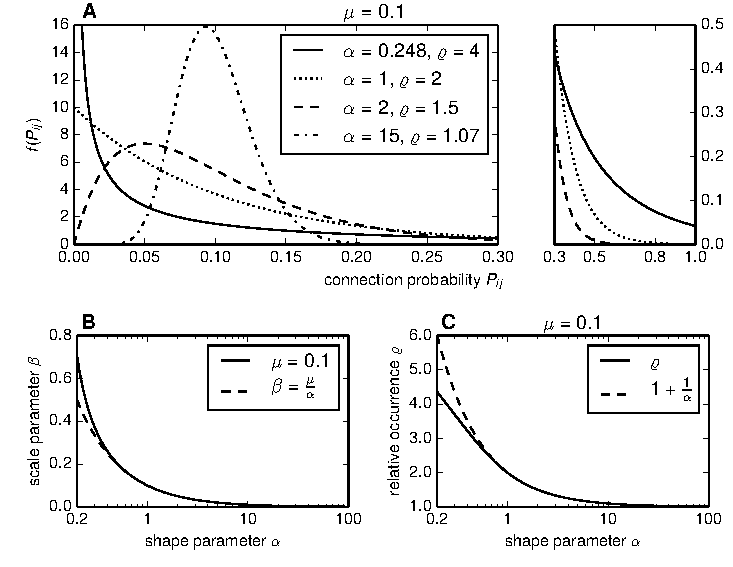
\includegraphics[width=\textwidth]{%
  %../figures/gamma_distribution/gamma_figure.pdf}
  img/gamma_figure.pdf}
\caption{Relative occurrence of bidirectional connections $\varrho$ in
  networks with gamma distributed connection probabilities. \textbf{A}
  Probability density functions of the truncated gamma distribution
  $\Gamma^T(\alpha,\beta)$ for different shape parameters $\alpha$ and
  the induced relative overrepresentation $\varrho$ in a network with
  such distributed connection probabilities $P_{ij}$. For given
  $\alpha$, the scale parameter $\beta$ was chosen such that $\mu =
  0.1$. Plot to the right continues the density functions on a
  different scale. \textbf{B} Contour of $\alpha$, $\beta$ pairings
  that yield an overall connection probability of $\mu =
  0.1$. \textbf{C} Relative occurrence $\varrho$ in dependence on
  $\alpha$ for fixed $\mu = 0.1$. For $\alpha \geq 1$ this
  relationship is well approximated by $\varrho \approx 1 +
  \frac{1}{\alpha}$.}
\label{fig:gd}
\end{figure}

%% In Figure~\ref{fig:gd} probability density functions for multiple
%% parameter sets $(\alpha, \beta)$ are shown. The rate parameter $\beta$
%% is determined by the given $\alpha$ and $\mu = 0.1$ through the
%% relation in \eqref{eq:gd3}. [Comment: I'm not sure it's worth deriving
%%   an expression for $\beta$. A good approximation is $\beta =
%%   \frac{\mu}{\alpha}$, ($K_{\alpha,\beta} = 1$). I just need to make
%%   it clear what I'm doing.]


%% The narrower the probability density around the mean $\mu = 0.1$ the
%% smaller is the expected overrepresentation of bidirectional
%% connections $\varrho$ in the network. To achieve a high $\varrho$ many
%% pairs with a high connection probability are needed. The dashed line
%% in Figure~\ref{fig:gd} marks the probability density function of the
%% probability distribution of connection probabilities $P_{ij}$ that
%% induce an overrepresentation of reciprocal pairs of $\varrho = 4$ as
%% found by \textcite{Song2005} leading to a highly skewed distribution
%% with a long tail. The relevance of such a distribution for cortical
%% networks however is debatable, as most connections are with a high
%% certainty not established seemingly wasting the network's potential
%% for different possible configurations.


%% Notably, to achieve an overrepresentation of $\varrho = 4$ as found by
%% \textcite{Song2005} most of the pairs in the network are almost
%% certainly unconnected .


%References: \href{http://herbsusmann.com/distributions/gamma-distribution-variance-proof.html}{Proof $\E(X^2)$}, 

